\documentclass{llncs}

% A. Objectives
%    1. You should apply one of the techniques studied in the course to
%       solve this problem.
%    2. Devise and perform an empirical evaluation of your system.
%    3. Report your work.
%    4. All your documentation and source code should be available on your GitLab
%       project repository, as well as tasks and milestones. This will be part of
%       the evaluation.
%
% B. Deliverables
%    1. Progress report (by the end of May) describing
%     - selected approach and
%     - general project work plan
%     - group presentation of the report
%    2. Project report
%     - description of the problem
%     - updated material from the progress report
%     - description of your approach
%     - description of the software: installation, requirements and usage notes
%     - empirical evaluation
%    3. Software
%     - application and required libraries/software
%     - brief installation notes (README file)
%    4. Final Presentation
%     - description of your approach
%     - strengths and weaknesses
%     - empirical evaluation
%     - contribution of team members
%
% C. Timeline
%    1. 2018-05-30 Progress report and presentation
%    2. 2018-06-18 Software deliverable and final report
%    3. 2018-06-22 Final Presentation and Demo

\usepackage[utf8]{inputenc}
\usepackage[T1]{fontenc}
\usepackage[english]{babel}

\usepackage{hyperref}
\usepackage{bookmark}
\usepackage{csquotes}

\usepackage{tikz,comment}
\usetikzlibrary{shapes.multipart,positioning,backgrounds}

\newcommand{\htw}{\emph{Hunt the Wumpus }}

\title{Hakuna Matata: A Logic-Based Agent for the \htw Game}
\subtitle{Project Report}
\author{Team White\\[2mm]Filippo~De~Bortoli \and Aneta~Koleva \and Lorenz~Leutgeb}
\institute{Free University of Bozen-Bolzano\\[3mm] \texttt{\{\href{mailto:filippo.debortoli@stud-inf.unibz.it}{filippo.debortoli},\href{mailto:aneta.koleva@stud-inf.unibz.it}{aneta.koleva},\href{mailto:lorenz.leutgeb@stud-inf.unibz.it}{lorenz.leutgeb}\}\newline @stud-inf.unibz.it}}

\begin{document}

\maketitle

\begin{abstract}
  The assigned task is to develop an intelligent agent that plays the \htw game, by using a logic-based approach in its implementation.
  In order to complete a run of the game, this agent has to be able to face several challenges, like the incompleteness of the available information about the state of the world or the search for the best strategy to employ.
  The chosen approach is to develop a hybrid agent that relies on an ASP core to actuate its strategy and on graph-theory techniques to obtain additional insights on how to proceed in the exploration of a dungeon.
  To assess the performance of our agent, we implemented an omniscient agent that obtains an optimal score for a given dungeon and we ranked our agent against it.
  In this report, we introduce our solution to this task, by detailing the architecture of the agent and describing the chosen strategy, the heuristics and the obtained results.
\end{abstract}

\section{Problem Statement}
%TODO Define what \htw is, all its rules and constraints.
%TODO Mention that it is also an example in the standard textbook AIMA and thus suited as an exercise in logic-based AI.

\htw is a single player, old computer game which was first released back in 1975. The game is played in the wumpus world(a cave) which is represented as a grid (default size 4x4) and in this world there are few challenges for the player. Each cell on the grid is a room which is connected by passageways with its orthogonally adjacent cell and in one of these cells there is Wumpus, a beast that eats the player if he enters the room. The player has only one arrow, that's one opportunity for shooting the Wumpus. In addition, some of the rooms are bottomless pits and if the player wanders in these rooms it will stay trapped. The main goal of the player is while facing these challenges, to find the hidden gold and leave the cave alive. At the beginning of the game, the player is always positioned on cell [1,1], facing to the right and has 0 points. From here it can use three moves : \textit{Forward, TurnLeft, TurnRight} for discovering its environment and three actions \textit{Shoot, Grab} and \textit{ Climb} for shooting the arrow, grabbing the gold and climbing out of the cave respectively. For each of the moves and actions the player loses 1 point and 10 points when using the arrow. When eaten by the wumpus or trapped in pit, loses 1000 points, and for climbing out of the cave with the gold gains 1000 points. Whenever the player goes to a new cell, it has five sensors that give information about:
\begin{description}
	\item [$\bullet$] Stench - whether the Wumpus is in adjacent cell 
	\item [$\bullet$] Breeze - whether there is a pit in adjacent cell	
	\item [$\bullet$] Glitter - when the gold is in the current cell
	\item [$\bullet$] Bump - whether the player has hit a border
	\item [$\bullet$] Scream- whether the Wumpus is hit by the arrow 
\end{description}
The locations of the gold and the wumpus are chosen randomly with uniform distribution in each cell other then the start. Additionally each cell can be a pit with probability 0.2.

In the book Artificial Intelligence: A Modern Approach, the game is used as an example for representing knowledge-based agents. The environment which represents the Wumpus World is is described as discrete, static, single-agent and partly-observable. For an agent in such environment the main challenge is its initial ignorance of the configuration of the world and using logical reasoning can be helpful for solving this. 



\section{Approach}
% This should be a high-level section that does not really talk too much
% about code (for that we have the "Implementation" section), but instead
% about the general approach.
\subsection{ASP technique}
For the purpose of this project, we decided to implement an intelligent agent that plays the wumpus game using ASP technique in combination with graph-theory techniques to explore the search space and find its best strategy for finishing the game with maximum points. The environment in which the agent is playing is discrete and static, since the wumpus, the gold and the pits are all fixed. The agent's initial knowledge base contains the rules of the game without specifying the size of the grid. The size is discovered by the agent when it hits a border and the 'Bump' percept is on, after which the agent knows how big the search space it is. In order to be able to find the best strategy, the agent first needs to acquire certain knowledge about the search space and to be able to reason wrt this knowledge. The facts and rules in the knowledge base are specified as ASP rules and DVL solver is used for grounding and solving. One of the advantages of ASP is the fact that it uses non-monotonic reasoning and closed world assumption which allow the agent to correctly derive what is logically right from it's knowledge base. Moreover DLV is able to process incomplete knowledge which the agent has while overcoming its initial ignorance with logical reasoning. 

%TODO Justify why we chose ASP (non-monotonic reasoning, fits nicely with incomplete knowledge), previous experience with it, easier to write high-level logic thanks to grounding. 
% maybe mention that we can write strong constraints, not sure if still have that

\subsection{A* search algorithm}
For better exploration of the world, we build a graph that represents reachability (with cost) for all cells. Then we use \textit{Manhattan distance} as a cost function for calculating the cost from the current cell to the next cell. 
For calculating the minimal cost of reaching the goal cell we use \textit{A* search algorithm} : \(f(n) = g(n) + h(n)\).
In our program \(g(n)\) represents the cost of the path from the current cell to the next cell \(n\), and \(h(n)\) represents the heuristic estimated cost of the cheapest path from cell \(n\) to the goal cell.  

%TODO How does our agent explore the world (A*-search)
%not sure if here should be explained the purpose of pathTurnCost,
%departureTurnCost and rotCost or leave that for implementation

\subsection{Different modes}
While playing, our agent can be in 1 from 4 available modes at any time. When the game starts, the first mode of the agent is \textit{explore}. It stays in this mode until it discovers the gold or there are cell which haven't been explored yet. Once the agent is in the cell where the gold is, its next action is to grab the gold and in this moment is in mode \textit{grab}. If there are no more cells safe for exploration, the gold is not grabbed and the agent is facing the wumpus, the mode switches to \textit{kill}. The last available mode is \textit{escape}, in which the agent is if it's not in any of the other three modes. The agent is in this mode after grabbing the gold or after not being able to explore any other cells and leaves the cave empty handed.

%TODO Describe the modes that we extracted from the gameplay and what are the conditions that make the agent switch modes.


%TODO Describe the high level approach


\begin{center}
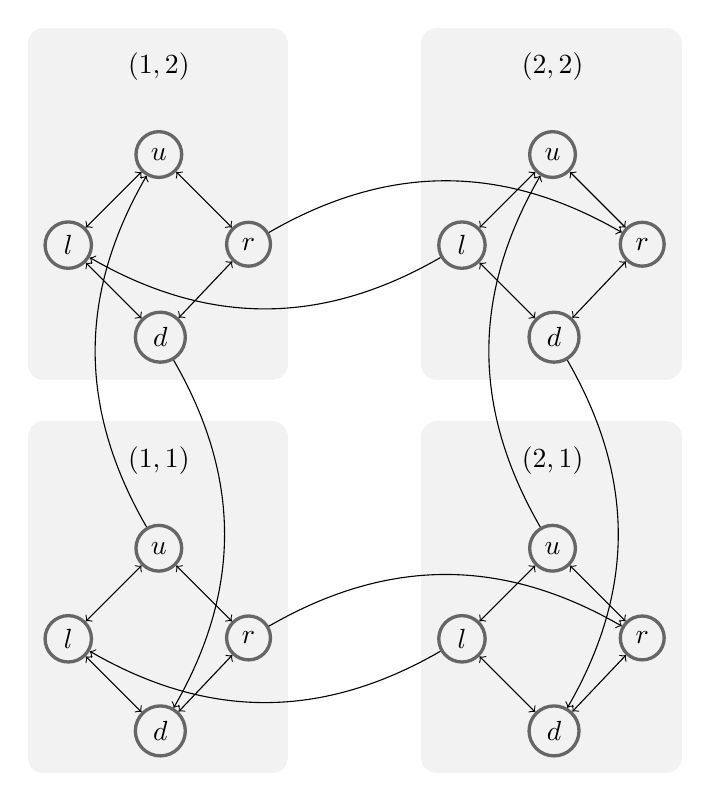
\begin{tikzpicture}[roundnode/.style={circle, draw=black!60, very thick,minimum size=4mm}]
	\begin{scope}
	    \node (n11) {$(1, 1)$};
		\node[roundnode] (u11) [below=5mm of n11] {$u$};
		\node[roundnode] (l11) [below left=10mm of u11] {$l$};
		\node[roundnode] (r11) [below right=10mm of u11] {$r$};
		\node[roundnode] (d11) [below right=10mm of l11] {$d$};
		\draw [<->] (u11) -> (l11);
		\draw [<->] (u11) -> (r11);
		\draw [<->] (d11) -> (l11);
		\draw [<->] (d11) -> (r11);
	\end{scope}

	\begin{scope}[xshift=5cm]
	    \node (n21) {$(2, 1)$};
		\node[roundnode] (u21) [below=5mm of n21] {$u$};
		\node[roundnode] (l21) [below left=10mm of u21] {$l$};
		\node[roundnode] (r21) [below right=10mm of u21] {$r$};
		\node[roundnode] (d21) [below right=10mm of l21] {$d$};
		\draw [<->] (u21) -> (l21);
		\draw [<->] (u21) -> (r21);
		\draw [<->] (d21) -> (l21);
		\draw [<->] (d21) -> (r21);
	\end{scope}

	\begin{scope}[yshift=5cm]
	    \node (n12) {$(1, 2)$};
		\node[roundnode] (u12) [below=5mm of n12] {$u$};
		\node[roundnode] (l12) [below left=10mm of u12] {$l$};
		\node[roundnode] (r12) [below right=10mm of u12] {$r$};
		\node[roundnode] (d12) [below right=10mm of l12] {$d$};
		\draw [<->] (u12) -> (l12);
		\draw [<->] (u12) -> (r12);
		\draw [<->] (d12) -> (l12);
		\draw [<->] (d12) -> (r12);
	\end{scope}

	\begin{scope}[yshift=5cm,xshift=5cm]
	    \node (n22) {$(2, 2)$};
		\node[roundnode] (u22) [below=5mm of n22] {$u$};
		\node[roundnode] (l22) [below left=10mm of u22] {$l$};
		\node[roundnode] (r22) [below right=10mm of u22] {$r$};
		\node[roundnode] (d22) [below right=10mm of l22] {$d$};
		\draw [<->] (u22) -> (l22);
		\draw [<->] (u22) -> (r22);
		\draw [<->] (d22) -> (l22);
		\draw [<->] (d22) -> (r22);
	\end{scope}

	\path [->] (r11) edge [bend left] (r21);
	\path [->] (l21) edge [bend left] (l11);
	\path [->] (u11) edge [bend left] (u12);
	\path [->] (d12) edge [bend left] (d11);
	\path [->] (u21) edge [bend left] (u22);
	\path [->] (d22) edge [bend left] (d21);
	\path [->] (r12) edge [bend left] (r22);
	\path [->] (l22) edge [bend left] (l12);

	\begin{pgfonlayer}{background}
		\filldraw[line width=4mm,join=round,black!5]
			(n11.north -| r11.east) rectangle (d11.south -| l11.west)
			(n21.north -| r21.east) rectangle (d21.south -| l21.west)
			(n12.north -| r12.east) rectangle (d12.south -| l12.west)
			(n22.north -| r22.east) rectangle (d22.south -| l22.west);
	\end{pgfonlayer}
\end{tikzpicture}
\end{center}

\section{Implementation}
%TODO Short section where we describe the system, referring to the appendix (see below)
%TODO as well as that we used DLV.

%TODO Generate and include the Dependency Graph

%TODO Autopilot (if it works at some point)

%TODO Refer to usage file for actually running the system.

\section{Evaluation}

%TODO mention that we used randomly generated instances:

\begin{tabular}{ccc}
$n$ & $N_n$ \\
4 & 120 \\
5 &  20 \\
6 &  20 \\
7 &  20 \\
8 &  20 \\
\end{tabular}

%TODO maybe more instances?

%TODO We implemented an agent that solves the instances with perfect information to compare against.

%\section{Introduction}

% TODO
%
% - describe the task that has been solved
% - outline structure of the report 
%\section{Installation and Usage}
\label{sec:usage}

\subsection{An example}
%\input{sections/strategy}
%\section{Evaluation}

% TODO
%
% - describe the structure of the test suite
% - is it necessary to describe machine specs for tests run?
%    I don't think so, we are not checking CPU time or machine-related data. ~Filippo
% - describe collected data (variables, clauses, models, ...)
% - desiderata: plot describing evolution of different versions of the front-end
% - arrogant: comparisons with data from other teams on same test suite.

%TODO Appendix: ASP Lite rendered as TeX from Markdown.

\end{document}
